\chapter{Experimental Setup}
in this chapter, we describe the Experimental setup, explain the design choices that went into adapting, building and evaluating our methods, starting with the agent scaffold, the Mlebench benchmark and the implemented ITS strategies

This chapter details the comprehensive methodology employed in this research, encompassing the experimental setup, the design choices made in adapting and building upon existing frameworks, and the specific procedures for evaluating the proposed inference-time scaling (ITS) strategies. The primary objective is to establish a transparent, rigorous, and replicable evaluation framework capable of quantitatively assessing the impact of these ITS techniques when applied to open-source Large Language Models (LLMs) engaged in complex machine learning engineering tasks.

\section{AIDE: AI-Driven Exploration in the Code Space}
At the center of this work, and the most critical component in my experimental setup is the agent scaffold itself, For this research work, I am leveraging AI-Driven Exploration (Aide), an open source agent scaffold, developed by WecoAi (Schmidt et al., 2025). AIDE is specifically designed to automate the trial and error process in developing machine learning models, working iteratively to find a solution in a tree search manner, exploring the `Code space`. 

The core principle behind AIDE is to address the significant amount of time that engineers and scientists spend on iterative experimentation, rather than to focus on conceptualizing and innovating.  To achieve that, AIDE frames the entire machine learning engineering process as a code optimization problem, modeling the trial and error as a tree search within a space of potential code solutions, each node is a potential solution problem (i.e. a code script), and each edge is an attempt at improving/debugging that solution.

At its heart. and as many other agent scaffolds, AIDE is powered by Large Language Models (LLMs), typically a strong model like gpt4 or Claude. These LLMs are responsible for proposing new code, debugging existing scripts, or suggesting and improvement or refinement to promising solutions. AIDE then reuses and refines these solutions, effectively trading computational resources for improved performance. Essentially, AIDE is performing some sort of inference time scaling, but the scope and the level of this scaling is of high-level nature. The implementation of AIDE is publicly available, which was a key factor in its selection for this thesis, allowing integration of custom inference time scaling methods.

% \subsection{Core Components and Methodology of AIDE}
% Below is a breakdown of how AIDE operates as outlined in there original paper(shmidt et al)
% \begin{figure}
%     \centering
%     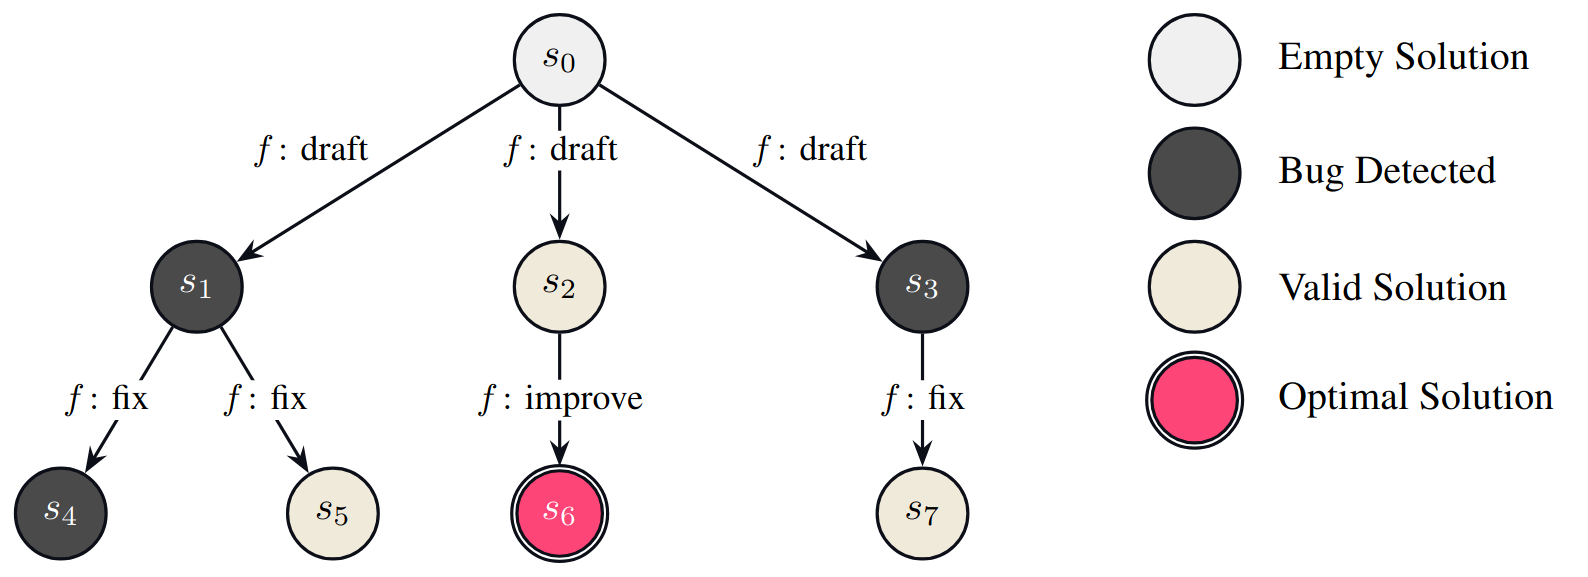
\includegraphics[width=0.8\linewidth]{images/aide-solution-tree.png}
%     \caption{A sample solution tree for AIDE, illustrating the drafting, fixing, and improvement steps. (Source: Schmidt et al., 2025, p. 4)}
%     \label{fig:enter-label}
% \end{figure}

% The Solution Tree ($T$): This is all discovered/proposed solutions (Python code scripts) and the improvement attempts (edges linking them) stored in a tree structure. The root solution ($s_0$) is typically an empty script, a node with value 'None'.

% Evaluator ($h$): This is a stateless function that takes a solution script as input and returns a scalar score (e.g., validation accuracy, loss). This score guides the search process. this evaluator is composed of a code interpreter that executes the code, then another LLM then takes the execution result (the trace back) and produces a structured output via function calling. this particular role is considered stateless since it always produce the same score, and it does not include past attempts in its evaluation, and this is important in the overall tree search for the best solution as every node or possible solution is evaluated primary on this.

% Search Policy ($\pi$): AIDE uses a simple, hard-coded search policy that determines the next step or next action. Based on the current state of the solution tree, it decides to:

% 1. Draft a new initial solution (if a desired number of diverse starting points hasn't been reached).

% 2. Debug a buggy node (if it's within a certain debug depth).

% 3. Improve an existing, non-buggy solution (typically targeting the current best-performing one).

% This policy has practical heuristics, such as initially exploring diverse solutions and then iteratively refining the most promising ones, while also limiting attempts to fix persistently broken solutions. Although this might be the most obvious area of improvement in the AIDE pipline, weather that was using a learned model that guides this search, the nature of the problems that small open source models have is largely not caused by the search heuristic, rather it is more fundamental in terms of ability to generate valid code in the first place, or correct usage of libraries and APIs.

% Coding Operator ($F$): This is the LLM itself as it proposes new scripts. It has three main entry points, each with specialized prompts:

% Drafting: Create a completely new solution `exploration`. The LLM is prompted to outline a plan to solve the problem (e.g., specify a neural network architecture and feature engineering ideas) and then generate a single-file Python program implementing that plan. These are then separated using regular expressions.

% Debugging: Repairing buggy solutions by inspecting error logs and execution traces. It attempts to fix issues like broken imports or incorrect tensor dimensions while preserving the overall approach.

% Improving: Called when a valid, non-buggy solution exists but could benefit from modifications (data preprocessing changes, architectural adjustments, or optimization tweaks and hiperparameter tuning). The LLM is prompted to propose a single `atomic` change, such as switching an optimizer or adding a regularization technique, so its impact on performance can be directly measured.

% Finally, to manage the LLM's context window and avoid `prompt explosion' from an  the growing history being fed to the model during the debugging and improvement phases, AIDE uses a summarization operator. Instead of appending all historical logs, this operator selectively extracts relevant information from the solution tree, such as Performance metrics (accuracy, AUC-ROC, etc.), Hyperparameter settings from previous attempts, Relevant hints for debugging (e.g., misaligned array shapes from trace-backs), This concise summary allows each code revision to be somewhat stateless yet guided by prior information, maintaining efficiency.

% Data Preview in Coding Prompts: AIDE also includes a small, static `data preview' in its coding prompts, providing the LLM with basic knowledge of the dataset's size or feature layout without needing extensive exploratory data analysis (EDA) at each step. As there is a code interpreter part of this iterative process, this Data preview tells the model exactly where and how the data is organized, and where to save its output or `submission.csv`

% The choice of AIDE as the foundational scaffold for this research is deliberate. It is open-source , it allows for the modification and integration of the inference-time scaling methods (self-consistency and self-reflection, etc) that are central to our work. Furthermore, AIDE's design, which explicitly models ML engineering as an iterative code optimization and tree search process powered by an LLM, provides a structured environment to study the effects of these techniques. It is established and proven to work effectively in solving ML tasks, as demonstrated in its original paper and subsequent evaluations on benchmarks like MLE-Bench, offers a great platform for experimentation. 

% AIDE has been tested and evaluated only using lagre-scale propriety LLMs, and our aim is to investigate how inference-time strategies can enhance AIDE's problem-solving capabilities, particularly its ability to make an open source, small-scale LLM generate more robust and higher-performing solutions on the challenging task like Machine learning Engineering.


% \section{MLE-Bench}
% To assess the performance of the enhanced aide scaffold we developed, we utilize the newly released MLE-bench, a benchmark for measuring how well AI agents perform at machine learning engineering, it is composed of 75 kaggle competitions, curated carefully from the Metakaggle dataset that contains around 5000 Kaggle competitions.
% This benchmark is designed specifically to be a benchmark for evaluating the performance of AI agents at machine learning engineering. MLE-Bench vary in category, scale, and complexity. This benchmark is designed not merely to test isolated skills, but to measure an agent's capacity for autonomous, end-to-end problem-solving—a workflow that spans model creation, training, evaluation, and iterative refinement.

% While MLE-Bench is a recent development, it is built upon a foundation of prior work aimed at evaluating LLMs coding and agentic abilities. Benchmarks like APPS (Hendrycks et al., 2021) and early evaluations of models such as Codex (Chen et al., 2021) have been used to measure general coding competence. The choice of MLE-Bench, and its particular relevance to this thesis, lies in its focus on tasks that are both representative of modern industry practices and known to be challenging for current AI systems, it offers a more specialized and demanding evaluation. However, it is very big benchmark, and evaluating on the 75 competitions is computationally infeasable for this thesis, hece, we opted for a subset of the benchmark,
% The core design of MLE-Bench is mostly around its task selection. The 75 selected competitions present an extremly difficult challenge for any coding agent. Essentially, MLE-Bench provides an offline Kaggle competition environment. For context, Kaggle is a platform that hosts data science and ML competitions where participants build predictive models to solve real-world challenges, competing for the best score on predefined metrics and earning rankings on a leaderboard. Top performers are often awarded monetary prizes, in addition to recognition with a bronze, silver, or gold medals. MLE-Bench adopts a similar structure to Kaggle, allowing for a realistic comparison of agent performance against historical human achievements 'offline leaderboard. The final results in this benchmark are often presented in terms of the average number of medals an agent would have won, determined by comparing its solution's metric on an unseen test set against the saved leaderboard from the original Kaggle competition.



% \section{Experiment Setup}

% To provide a rigorous and reliable evaluation of the inference-time strategies proposed in this thesis, a carefully designed experimental setup is essential. This section outlines the benchmark competitions, the baselines for comparison, the specific metrics used for evaluation, and the overall experimental procedure. The primary goal is to establish a solid evaluation framework that can take a given agent configuration as input and produce clear, quantitative metrics to determine its effectiveness relative to other methods.

% 1. Benchmark Competitions

% The foundation of our evaluation is a representative subset of competitions from the official MLE-Bench framework. While the full MLE-Bench is extensive, running experiments on all 75 competitions is computationally prohibitive for this project. Therefore, I have selected a curated subset of 10 competitions from the 'lite' complexity category. This choice was driven by several factors:

% Diversity: The selected competitions span 6 distinct machine learning categories, ensuring that our evaluation is not biased towards a single problem type. This diversity is crucial for assessing the general applicability of the proposed inference strategies.

% Feasibility: By focusing on 'lite' competitions, which are relatively lightweight in terms of data size and complexity, our experiments can focus on the quality of the agent's problem-solving process rather than being constrained by the technical overhead of handling massive datasets.

% Representativeness: This subset is a good representation of the full 'lite' category and provides a strong, empirical basis for evaluation.

% Flexibility: The chosen set is flexible enough to be extended in future work, either by including more competitions from the 'lite' category for a full standard comparison or by adding selected 'medium' complexity tasks to further test the limits of our methods.

% The 10 competitions selected for this benchmark are detailed in Table \ref{tab:competitions}.

% % \begin{table}[h!]
% % \centering
% % \caption{Selected Benchmark Competitions from MLE-Bench 'Lite' Category}
% % \label{tab:competitions}
% % \begin{tabular}{ll}
% % \hline
% % \textbf{Competition Name} & \textbf{Category} \ \hline
% % aerial-cactus-identification & Image Classification \
% % leaf-classification & Image Classification \
% % spooky-author-identification & Text Classification \
% % random-acts-of-pizza & Text Classification \
% % tabular-playground-series-may-2022 & Tabular \
% % nomad2018-predict-transparent-conductors & Tabular \
% % denoising-dirty-documents & Image to Image \
% % text-normalization-challenge-english-language & Sequence to Sequence \
% % text-normalization-challenge-russian-language & Sequence to Sequence \
% % mlsp-2013-birds & Audio Classification \ \hline
% % \end{tabular}
% % \end{table}

% 2. Baselines for Comparison

% To properly contextualize the performance of our proposed methods, we will benchmark them against a diverse set of established baselines. The aim is twofold: first, to prove that our strategies provide a meaningful improvement over a standard open-source model, and second, to demonstrate that these strategies make open-source models competitive with both closed-source counterparts and human experts.

% The baselines are summarized in Table \ref{tab:baselines}.

% % \begin{table}[h!]
% % \centering
% % \caption{Baselines for Performance Comparison}
% % \label{tab:baselines}
% % \begin{tabular}{lll}
% % \hline
% % \textbf{Baseline} & \textbf{Type} & \textbf{Reason for Inclusion} \ \hline
% % \textbf{AIDE + GPT-4o} & CS / High-Capability & Represents a strong, widely-used frontier model. \
% % & & Provides a high-water mark for performance. \ \
% % \textbf{AIDE + o4-mini} & CS / Reasoning-Optimized & Assumed to be a cost-effective, state-of-the-art reasoning \
% % & & model from OpenAI. Serves as a key SOTA reference. \ \
% % \textbf{AIDE + Llama 3.1 (405B)} & OS / High-Capability & A top-tier open-source model. Outperforming this \
% % & & demonstrates the power of our strategy. \ \
% % \textbf{Our Model + Default AIDE} & OS / Ablation & \textbf{Critical baseline.} This isolates the performance gain \
% % & & attributable specifically to our inference strategies, \
% % & & by removing them from our chosen model. \ \
% % \textbf{Human Performance} & Human Eval & Provides real-world context by comparing agent scores \
% % & & to the original Kaggle leaderboards. \ \hline
% % \end{tabular}
% % \end{table}

% 3. Evaluation Metrics

% To capture a holistic view of agent performance, we will use a suite of metrics inspired directly by the MLE-Bench and AIDE papers. These metrics evaluate an agent's ability to produce functional code, understand the task requirements, and ultimately generate an optimal solution.

% Code and Submission Generation: These metrics assess the fundamental ability of the agent to generate working code and complete the task.

% Valid Code Rate (\%): The number of steps that produce a valid, executable script divided by the total number of steps, averaged across seeds and competitions. A higher rate indicates a stronger fundamental code generation capability.

% Valid Submission Rate (\%): The percentage of independent runs (i.e., per seed, per competition) that successfully produce a submission file that passes the benchmark's validity checks. This is a stricter measure of task completion.

% Performance Against Human Baselines: Once a valid submission is produced, its quality is scored against the historical human leaderboard.

% Above Median (\%): The percentage of competitions where the agent's best score is strictly better than the median score achieved by human participants.

% Any Medal (\%): The percentage of competitions where the agent's best score is high enough to have earned a bronze, silver, or gold medal according to official Kaggle rules. This is our headline metric for overall success.

% The final results for each agent configuration will be presented in a summary table, as shown in the template in Table \ref{tab:results_template}.

% % \begin{table}[h!]
% % \centering
% % \caption{Template for Aggregated Results Table}
% % \label{tab:results_template}
% % \begin{tabular}{lccc}
% % \hline
% % \textbf{Model + Method} & \textbf{Valid Submission (\%)} & \textbf{Above Median (\%)} & \textbf{Any Medal (\%)} \ \hline
% % AIDE + o4-mini & X% 
% % ±
% % ±
% %  Y & X% 
% % ±
% % ±
% %  Y & X% 
% % ±
% % ±
% %  Y \
% % Our Model + Strategy 1 & X% 
% % ±
% % ±
% %  Y & X% 
% % ±
% % ±
% %  Y & X% 
% % ±
% % ±
% %  Y \
% % Our Model + Default AIDE & X% 
% % ±
% % ±
% %  Y & X% 
% % ±
% % ±
% %  Y & X% 
% % ±
% % ±
% %  Y \ \hline
% % \end{tabular}
% % \end{table}

% 4. Experimental Procedure

% To ensure a fair and repeatable evaluation, all experiments are conducted using a standardized protocol within a consistent environment.

% Environment: All runs are executed within a Dockerized environment to ensure consistency. AIDE is configured with fixed hyperparameters for all methods (e.g., 20 steps per attempt, 5 initial drafts).

% Execution: For each of the 10 competitions, every agent configuration ("Method") is run for k=3 independent attempts (seeds). This helps account for the inherent stochasticity of LLMs.

% Data Collection: After each run, we automatically collect the raw data, including whether a valid submission was generated and its corresponding score.

% Metric Calculation: Using the collected data, we calculate the flags for Valid Submission, Above Median, and Any Medal for each run.

% Aggregation: These flags are then aggregated. For metrics like Above Median and Any Medal, we consider a competition "solved" if at least one of the three seeds was successful (a pass@3 approach). The final percentages are averaged across the 10 competitions, with results reported as mean ± standard error.

% This standardized pipeline ensures that as we introduce and test new inference-time strategies, the results are directly and fairly comparable to our established baselines.



% % This is essentially what AIDE’s “solution tree” does conceptually – it navigates a solution space tree by proposing variations and seeing which yields better scores. Another formulation is the Tree-of-Thoughts
% % approach (Yao et al., 2023) where the model can propose multiple thoughts (steps of a solution)

% % This is somewhat what AIDE does by default (running the full training code to get a score), but one could go further and allow fine-grained tool use: the agent could execute just a part of the code (say a data pre-processing step) to inspect intermediate results, or call a library function to check documentation, etc. Another tool is a web browser or documentation fetcher, useful if the coding problem needs external knowledge
% % (though MLE-bench specifically disallows internet to prevent cheating). Still, 

% % For instance, in
% % OpenAI’s tests, they tried different “scaffolds”: AIDE, ResearchAgent, CodeAct, etc., each of which
% % structures the LLM’s process differently. 

% % AIDE’s self-reflection is essentially
% % an internal critic role given to the same model. We could also have a different model entirely
% % serve as the critic – for instance, use a 13B model to generate code and a more reliable 13B or
% % a set of heuristic rules to review it. This two-model system was not explicitly used in AIDE (to
% % our knowledge, AIDE uses one model for everything), but it’s a viable ITS approach: compose
% % multiple smaller experts rather than rely on one monolith. Each expert at inference time does
% % part of the task. 

% % search algorithms to explore solution space, tool use to gain information or verify outputs during generation, and modular agent frameworks that break the task into
% % pieces handled sequentially. These methods have proven effective: for example, using a Process Reward
% % Model + search enabled a 3B model to outperform a 70B model on a math benchmark, and
% % self-debugging allowed models to fix errors that they would otherwise miss. Importantly, most of these
% % techniques do not require fine-tuning the base model – they work by manipulating the inference
% % process (through prompting, iterating, or orchestration). Some advanced methods do introduce learned
% % components (e.g. training a verifier network, or fine-tuning the model to better utilize reflections), which blurs the line between pure inference-time and training. We’ll discuss a few such cases as well, but
% % the primary focus is on what can be done on the fly with an off-the-shelf model. The ultimate goal of
% % 5these strategies is well captured by OpenAI’s notion of “self-verification”, where the model can reliably
% % check its own work instead of relying on a giant ensemble or an external judge. In the next section,
% % we propose concrete techniques from these categories that AIDE could adopt to further empower its
% % small-model code generation in the ML domain.
% % **EITHER SPEAK ABOUT AIDE AND MLE BENCH HERE OR IN THE METHODS SECTINO**